\section{Apache JMeter}

JMeter is a desktop application, designed to test and measure the performance and functional behavior of applications. JMeter works  as the "client side" of a "client/server" application. It measures response time and all other server resources such as CPU loads, memory usage, and resource usage. In this respect, JMeter can be used effectively for functional test automation. The software features FTP and HTTP requests and extensible custom scripting features \cite{Nevedrov2007}.

The tool works in a hierarchical manner. The initial component of the tool is called Test Plan. Test Plan is the root element of the JMeter scripts and houses the other components, such as Threads, Config Elements, Timers, Pre-Processors, Post-Processors, Assertions, and Listeners. The Fig. \ref{fig:jmeteranatomy} presents an example of a JMeter script anatomy \cite{Erinle2013}.

\begin{figure}[!ht]
\centering
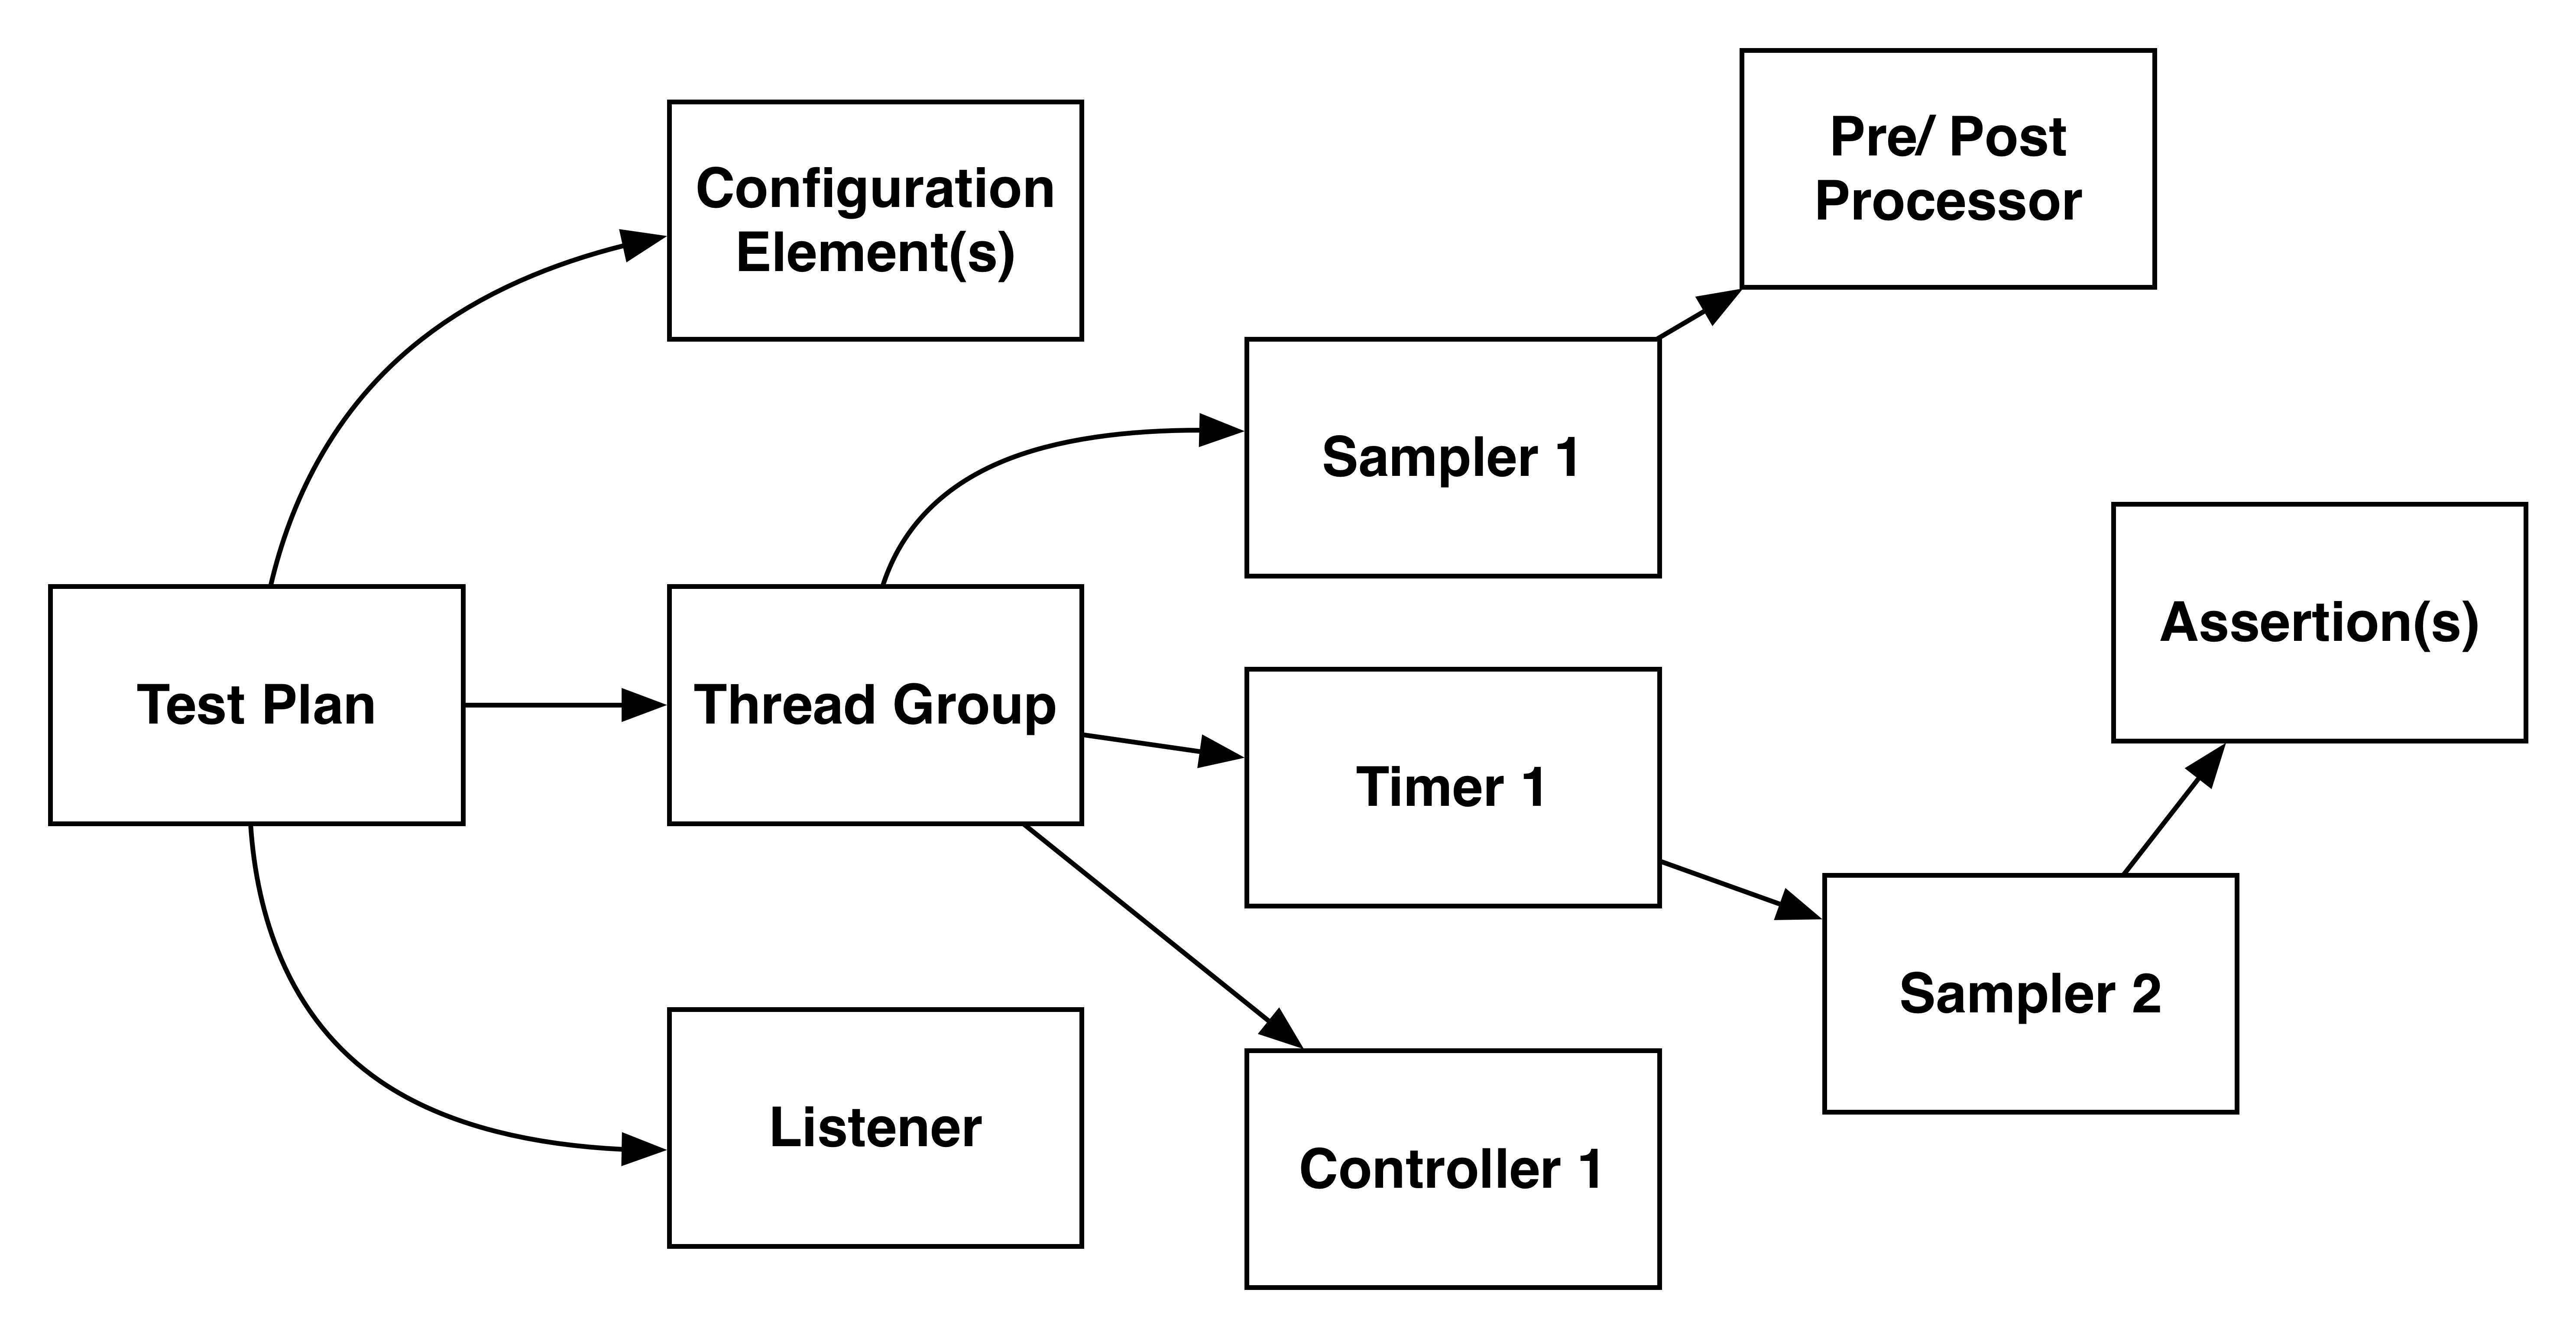
\includegraphics[width=0.5\textwidth]{./images/jmeteranatomy.png}
\caption{Anatomy of JMeter script \cite{Erinle2013}}
\label{fig:jmeteranatomy}
\end{figure}

Thread Groups represents the number of threads/users JMeter will use to execute the test plan. All controllers and samplers for a test must reside under a Thread Group. Other elements, such as listeners, may be placed directly under a test plan. Thread Group configurations provide options to specify the number of threads that will be used for the test plan, how long it will take for all threads to become active (ramp up), and the number of times to execute the test \cite{Erinle2013}.

Configuration elements work with a sampler, enabling requests to be modified or added to. Listeners are components  used to post process request data, storing the results of a test run making possible it to be further analyzed.  Listeners can be added anywhere in the test script, including directly under the test plan. They will collect data only from the elements at or below their level \cite{Erinle2013} \cite{Nevedrov2007} \cite{Halili2008}. 

Samplers allow JMeter to send requests to a server and wait for a response. Requests are processed in the order they appear in the tree. Timers allow JMeter   pause a certain amount of time before each sampler \cite{Nevedrov2007}  \cite{Halili2008}.

The main results presented by JMeter are:

\begin{itemize}
\item Response time : the elapsed time from just before sending the request to just after the last response has been received.
\item Latency: latency from just before sending the request to just after the first response has been received. Thus the time includes all the processing needed to assemble the request as well as assembling the first part of the response.
\item Connect Time: time it took to establish the connection, including SSL handshake. 
\item Median:  number which divides the samples into two equal halves. Half of the samples are smaller than the median, and half are larger. The Median is the same as the 50th Percentile.
\item 90\% Line (90th Percentile) is the value below which 90\% of the samples fall. The remaining samples too at least as long as the value. 
\item Standard Deviation:  measure of the variability of a data set. 
\end{itemize}